

\documentclass[../../tc_tp3_main.tex]{subfiles}

\begin{document}


\chapter{Filtro con GIC}

\section{Introducci\'on: el GIC}
\label{section:1-intro}


\todo[inline]{explicar:cuando se quiere hacer un filtro de segundo orden sin usar bobinas, usamos GIC para simular sus efectos} 


\begin{figure}[H]
	\centering
	\begin{circuitikz}
		\def\gicgxCenter{0}
		\def\gicgxGnd{3}
		\def\gicgyVin{0}
		\def\gicgyopamAp{0.5}
		\def\gicgyopamBo{2}
		\def\gicgyopamABm{3.5}
		\def\gicgyopamAo{5}
		\def\gicgyopamBp{6.5}
		\def\gicgyGnd{7}
		\def\gicgxOpamBin{-.5}
		\def\gicgxOpamAin{1}
		
		\draw
		(\gicgxCenter, -1)  node[ground] {}
		to [generic, l=$Z_5$] 		(\gicgxCenter, \gicgyopamAp) node[left]{$V_{GIC}$}
		to [generic, l_=$Z_4$]	(\gicgxCenter, \gicgyopamBo)  node[right]{$V_2$}
		to [generic, l_=$Z_3$]  	(\gicgxCenter, \gicgyopamABm)
		to [generic, l_=$Z_2$] 	(\gicgxCenter, \gicgyopamAo)  node[left]{$V_1$}
		to [generic, l_=$Z_1$] 	(\gicgxCenter, \gicgyopamBp)
		to [short, -o, i<=$I$] 			(\gicgxCenter, \gicgyGnd) node[above]{$V_{GIC}$} 
		
		(-1.5,5) node [op amp, rotate=180, xscale=0.7, yscale = 0.7] (opamB) {}
		(opamB.-) |- (\gicgxOpamBin, \gicgyopamABm) 
		to[short,-*]  (\gicgxCenter, \gicgyopamABm)
		(opamB.+) |- (\gicgxOpamBin, \gicgyopamBp) 
		to[short,-*]  (\gicgxCenter, \gicgyopamBp) 
		(opamB.out) |- (-2, \gicgyopamBo) 
		to [short,-*]  (\gicgxCenter, \gicgyopamBo)
		
		(2,2) node [op amp, xscale=0.7, yscale = 0.7] (opamA) {}
		(opamA.-) |- (\gicgxOpamAin, \gicgyopamABm) node[above]{$V_{GIC}$} 
		to[short, *-*]  (\gicgxCenter, \gicgyopamABm) 
		(opamA.+) |- (\gicgxOpamAin, \gicgyopamAp) 
		to [short,-*]  (\gicgxCenter, \gicgyopamAp)
		(opamA.out) |- (2, \gicgyopamAo) 
		to[short,-*]  (\gicgxCenter, \gicgyopamAo)
		
	;\end{circuitikz}
	\caption{GIC gen\'erico con \textit{op amps} ideales}
	\label{fig:ej1-gicg}
\end{figure}


Como consideramos ideales a ambos operacionales, la tensi\'on de entrada se encuentra replicada donde se encuentran los terminales inversores del circuito, y a su vez en la entrada no inversora del segundo operacional. Asimismo, como no hay corriente entre $V^+$ y $V^-$ para ninguno de los operacionales, hay s\'olo tres corrientes, puesto que la corriente de $Z_2$ es la misma que la de $Z_3$, y la de $Z_4$ que la de $Z_5$. Quedan definidas entonces las ecuaciones:


 \[
	\left\{
 	\begin{aligned}
		 \frac{V_{GIC} - V_1}{Z_1} - I &= 0\\
		\frac{V_{GIC} - V_1}{Z_2} + \frac{V_{GIC} - V_2}{Z_3} &= 0 \\ 
		\frac{V_{GIC} - V_2}{Z_4} + \frac{V_{GIC}}{Z_5} &= 0
	\end{aligned}
	\right.
 \]
 
 Sustituyendo hacia atr\'as, podemos obtener la transferencia hasta la salida de cada operacional:
 
\begin{equation}
	\label{eq:1-v1v2g}
	\left\{
 	\begin{aligned}
		\frac{V_1}{V_{GIC}} & =  -\frac{Z_2 \cdot Z_4}{Z_3 \cdot Z_5}\\
		\frac{V_2}{V_{GIC}} & =  1+ \frac{Z_4}{Z_5} \\ 
	\end{aligned}
	\right.
 \end{equation}
 
 
 
 De aqu\'i se puede despejar la impedancia de entrada del GIC, es decir $\frac{V_{GIC}}{I}$:
 
 \begin{equation}
 	\label{eq:1-z-gic-g}
 	Z = \frac{Z_1 \cdot Z_3 \cdot Z_5}{Z_2 \cdot Z_4}
 \end{equation}

De esta forma, combinando las impedancias convenientemente, se pueden obtener impedancias de toda \'indole (es decir, donde el n\'umero $Z$ puede estar te\'oricamente en cualquier punto del plano complejo). 





\section{Filtro a dise\~nar}


\begin{figure}[H]
	\centering
	\scalebox{0.8}{
		\begin{circuitikz}
			\def\cxin{-5}
			\def\cxC{-3}
			\def\cyC{5.5}
			\def\cxCenter{0}
			\def\cxGnd{3}
			\def\cyVin{0}
			\def\cyopamAp{0.5}
			\def\cyopamBo{2}
			\def\cyopamABm{3.5}
			\def\cyopamAo{5}
			\def\cyopamBp{6.5}
			\def\cyGnd{7}
			\def\cxOpamBin{-.5}
			\def\cxOpamAin{1}
			
			\draw
			(\cxCenter, -1)  node[ground] {}
			to [R, l_=$R_8$] 		(\cxCenter, \cyopamAp) node[left]{$V_{GIC}$}
			to [R, l_=$R_4$]		(\cxCenter, \cyopamBo)  node[right]{$V_{out}$}
			to [R, l_=$R_3$]  		(\cxCenter, \cyopamABm)
			to [C, l_=$C_2$] 		(\cxCenter, \cyopamAo)  node[left]{$V_1$}
			to [R, l_=$R_1$] 		(\cxCenter, \cyopamBp)
			to [short, -*] 		(\cxCenter, \cyGnd) node[above]{$V_{GIC}$} 
			
			(\cxCenter, \cyGnd) 
			to [short, *-*] (\cxC, \cyGnd) 
			to [R=$R_6$, *-o] (\cxin, \cyGnd) node[left] {$V_{in}$}
			
			(\cxC, \cyGnd)
			to [C = $C_6$] (\cxC,\cyC) node[ground] {}
			
			
			(-1.5,5) node [op amp, rotate=180, xscale=0.7, yscale = 0.7] (opamB) {}
			(opamB.-) |- (\cxOpamBin, \cyopamABm) 
			to[short,-*]  (\cxCenter, \cyopamABm)
			(opamB.+) |- (\cxOpamBin, \cyopamBp) 
			to[short,-*]  (\cxCenter, \cyopamBp) 
			(opamB.out) |- (-2, \cyopamBo) 
			to [short,-*]  (\cxCenter, \cyopamBo)
			
			(2,2) node [op amp, xscale=0.7, yscale = 0.7] (opamA) {}
			(opamA.-) |- (\cxOpamAin, \cyopamABm) node[above]{$V_{GIC}$} 
			to[short, *-*]  (\cxCenter, \cyopamABm) 
			(opamA.+) |- (\cxOpamAin, \cyopamAp) 
			to [short,-*]  (\cxCenter, \cyopamAp)
			(opamA.out) |- (2, \cyopamAo) 
			to[short,-*]  (\cxCenter, \cyopamAo)	
		;\end{circuitikz}
	}
	\caption{Esquema del circuito}
	\label{fig:ej1-circuito}
\end{figure}

El GIC que utilizaremos en este trabajo se obtiene con las siguientes sustituciones:

 \[
	\left\{
 	\begin{aligned} 
		Z_1 & =  R_1 \\
		Z_2 & =  \frac{1}{s\cdot C_2} \\
		Z_3 & =  R_3 \\
		Z_4 & =  R_4 \\
		Z_5 & =  R_8
	\end{aligned}
	\right.
 \]

Por lo tanto, reemplazando en la ecuaci\'on (\ref{eq:1-z-gic-g}) obtenemos la impedancia de este GIC:

 \begin{equation}
 	\label{eq:1-z-gic}
 	Z(s) = s\cdot \frac{R_1 \cdot R_3 \cdot R_8 \cdot C_2}{R_4}
 \end{equation}

Entonces, con esta secci\'on del filtro estamos emulando una bobina ideal de inductancia:
\begin{equation}
	\label{eq:1-LGIC}
	L_{GIC} = \frac{R_1 \cdot R_3 \cdot R_8 \cdot C_2}{R_4}
\end{equation}

La salida, sin embargo, se mide dentro del GIC. Trataremos a este sistema como la combinaci\'on en cascada de dos sistemas: de $V_{in}$ a $V_{GIC}$, y de $V_{GIC}$ a $V_{out}$.
  
  
  
\subsection{Transferencia de $V_{in}$ a $V_{GIC}$} 
 
Teniendo en cuenta el resultado obtenido en la ecuaci\'on (\ref{eq:1-z-gic}), podemos simplificar el circuito de la siguiente manera: 

\begin{figure}[H]
	\centering
	
	\begin{circuitikz}
		\def\rlcxin{-5}
		\def\rlcxC{-3}
		\def\rlcyC{5.5}
		\def\rlcxCenter{-1}
		\def\rlcyGnd{7}
		
		\draw
		(\rlcxCenter, \rlcyC)  node[ground] {}
		to [cute inductor, l_=$L_{GIC}$] 		(\rlcxCenter, \rlcyGnd)  node[above]{$V_{GIC}$} 
		to [short, *-*] (\rlcxC, \rlcyGnd) 
		to [R=$R_6$, *-o] (\rlcxin, \rlcyGnd) node[left] {$V_{in}$}
		
		(\rlcxC, \rlcyGnd)
		to [C = $C_6$] (\rlcxC,\rlcyC) node[ground] {}
	;\end{circuitikz}
	
	\caption{Reemplazo del GIC por su inductancia equivalente}
	\label{fig:ej1-rlc}
\end{figure}

La tensi\'on de salida de esta secci\'on, entonces, puede hallarse aplicando un divisor de tensi\'on entre la impedancia de entrada desde $V_{in}$ y del paralelo de la bobina y el capacitor. Se obtiene entonces que:

\begin{equation}
	\label{eq:1-vgicvin}
	\frac{V_{GIC}}{V_{in}}(s) = \frac{s\cdot \frac{L_{GIC}}{R_6}}{ L_{GIC}C_6 \cdot s^2  + \frac{L_{GIC}}{R_6} \cdot s + 1}
\end{equation}

 
 
 
\subsection{Transferencia de $V_{GIC}$ a $V_{out}$}

Para obtener esta transferencia, basta observar que lo que ahora llamamos $V_{out}$ es lo que en la introducci\'on llamamos $V_2$. Por lo tanto, reemplazando los valores gen\'ericos de la ecuaci\'on (\ref{eq:1-v1v2g}) por los particulares de este circuito, obtenemos que:

\begin{equation}
	\label{eq:1-voutvgic}
	\frac{V_{out}}{V_{GIC}} (s) = 1+\frac{R_4}{R_8}
\end{equation}

Por lo tanto, la funci\'on transferencia del circuito se obtiene haciendo el producto de las ecuaciones (\ref{eq:1-vgicvin}) y (\ref{eq:1-voutvgic}):

\begin{equation}
	\label{eq:voutvin}
	H(s) = \left( 1+\frac{R_4}{R_8} \right) \cdot \left(  \frac{s\cdot \frac{L_{GIC}}{R_6}}{ LC_6 \cdot s^2  + \frac{L_{GIC}}{R_6} \cdot s + 1} \right)
\end{equation}

Esto corresponde a un \textbf{filtro pasabanda}, definido por los siguientes parametros:

\begin{equation}
	\label{eq:1-w0QyHw0}
	\left\{
	 	\begin{aligned}
			\omega_0 &= \sqrt{\frac{1}{L_{GIC}C_6}}\\
			Q &= R_6 \cdot \sqrt{\frac{C_6}{L_{GIC}}} \\ 
			\abs{H(i\omega_0)} &= 1+\frac{R_4}{R_8}
		\end{aligned}
	\right.
 \end{equation}



\section{Dise\~no del filtro pasabanda}


\begin{figure*}[h!]
	\centering
  	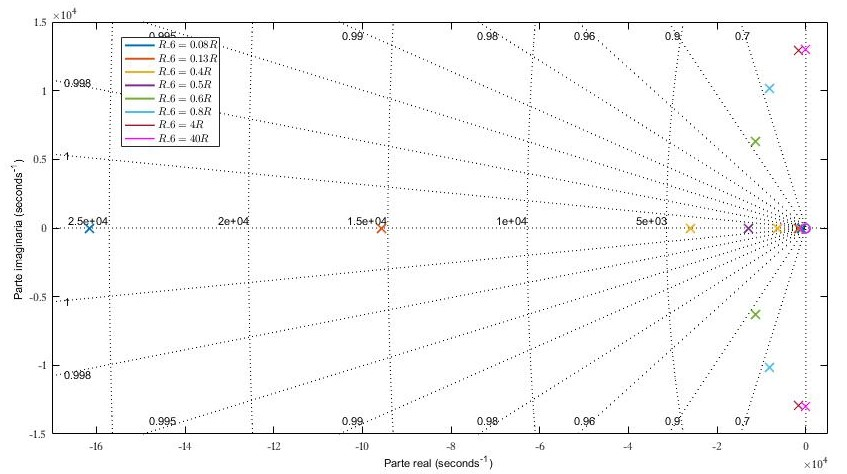
\includegraphics[scale = 0.7]{imagenes/polos.jpg}
  	\caption{Ubicaci\'on de los polos para distintos valores de $R_6$}
  	\label{fig:1-polos}
\end{figure*}



Las especificaciones de dise\~no de este filtro son:


\begin{equation}
	\left\{
		\begin{aligned}
			\omega_0 &= 13,000\nicefrac{rad}{s} & \Rightarrow f_0 = 2,079Hz \\
			Q &= 4  & \Rightarrow f_1 = 1,827Hz &\wedge f_1 = 2,344Hz  \\ 
		\end{aligned}
	\right.
 \end{equation}
 
El par\'ametro $\abs{H(i\omega_0)}$ no est\'a definido a priori. Sin embargo, se debe tener presente que el mismo corresponde a la salida de un \textit{op amp} en la frecuencia en la cual m\'as cr\'itico es que el circuito funcione correctamente. Por lo tanto, ser\'ia poco pr\'actico tener una gran ganancia en este punto, puesto que esto limitar\'ia mucho el rango de tensiones de entrada admisibles, ya que si bien en esta frecuencia el \textit{slew rate} no deber\'ia ser un problema, no ocurre lo mismo con la saturaci\'on. \par 
 
Para simplificar la elecci\'on de componentes, se establecen las siguientes relaciones entre los mismos: 
 
\begin{equation}
	\label{eq:1-relacionescomponentes}
	\left\{
		\begin{array}{ccccccccc}	
			R_1 &=& R_3 &=& R_4 &=& R_8 &=& R\\
			R_6 &=& Q\cdot R &=& 4 \cdot R \\
			C_2 &=& C_6 &=& C
		\end{array}
	\right.
 \end{equation} 
 
 Reemplazando en (\ref{eq:1-w0QyHw0}), se obtiene que:
 
 \begin{equation}
	\left\{
	 	\begin{aligned}
			\omega_0 &= \frac{1}{RC}\\
			Q &= 4\\ 
			\abs{H(i\omega_0)} &= 2
		\end{aligned}
	\right.
 \end{equation}
 
 Resulta entonces que, si se respeta el criterio establecido en (\ref{eq:1-relacionescomponentes}), s\'olo queda elegir $R$ de tal manera que los valores de $R_6 = 4\cdot R$ y $C = \frac{1}{13,000 \nicefrac{rad}{s} \cdot R}$ puedan obtenerse con el menor error posible con valores comerciales y est\'en en un rango razonable de valores. \par
 
 Para definir dicho rango de valores, se tomar\'a el siguiente criterio:
 
 \begin{itemize}
	\item  $R_6$ se encuentra en serie con la entrada del circuito, y por lo tanto se establecer\'a entre ella y la resistencia interna del generador un divisor de tensi\'on, cuyos efectos ser\'an despreciables s\'olo si $R_6 \gg R_G = 50\Omega$. Por lo tanto, $R_6$ debe ser al menos del orden de los $k \Omega$
	\item Puesto que el ruido t\'ermico es proporcional a la resistencia, no se utilizar\'an resistencias del orden de los $M\Omega$.
  	\item Las capacidades deben ser mucho mayores a las que introducen las puntas del osciloscopio al medir, que son de alrededor de $100pF$ si se utilizan en $\times 1$. Por ende, requeriremos que $C$ sea mayor a $10nF$, de forma que sea al menos 100 veces mayor que la del osciloscopio. 
 \end{itemize}


\subsection{Funci\'on de $R_6$}


Si consideramos la simplificaci\'on del circuito utilizada en la figura (\ref{fig:ej1-rlc}), $R_6$ es una resistencia serie en un circuito resonante. Como tal, su valor no influye en la frecuencia de resonancia, sino que determina el factor de calidad del circuito: a medida que $R_6$ se hace m\'as grande, el comportamiento del circuito se acerca m\'as a un pasabanda ideal, es decir uno con ancho de banda tendiendo a 0. An\'alogamente, a medida que $R_6$ se hace 0, el ancho de banda crece, convirtiendo al circuito en un pasa todo. \par

Esto se debe a que el factor de calidad del filtro $Q = \nicefrac{R_6}{R}$, donde $R$ lo consideramos constante, es inversamente proporcional a esta resistencia. Por lo tanto, para $R_6=0.5\cdot R$, el circuito tiene sus dos polos superpuestos en $s = -\omega_0$. A medida que aumenta, los polos se hacen complejos conjugados , acerc\'andose cada vez m\'as al eje imaginario, donde se encontrar\'ian los polos del pasabanda ideal. Si $R_6$ disminuye, en cambio, los polos se separan en dos reales distintos entre s\'i,   aumentando cada vez m\'as el ancho de banda del circuito. \par

Esto puede observarse en la figura (\ref{fig:1-polos}). De la misma podemos concluir que la resistencia $R_6$ es el componente que define la selectividad del filtro.



\subsection{Funci\'on de $R_8$}

La resistencia $R_8$ establece la conexi\'on entre los operacionales que integran el GIC y tierra. De no incluirse en el circuito, el GIC entero se comportar\'ia como un circuito abierto, y lo mismo si se reemplazara por un cable: la impedancia total del GIC se har\'ia 0. \par

Sin embargo, en este an\'alisis no se est\'a teniendo en cuenta las limitaciones de los operacionales. Si reemplazamos los valores gen\'ericos de las ecuaciones (\ref{eq:1-v1v2g}) con los particulares de este GIC, podemos observar qu\'e ocurre con la transferencia a cada operacional:

\begin{equation}
	\left\{
	 	\begin{aligned}
			\frac{V_1}{V_{GIC}} &= -\frac{R_4}{R_8} \cdot \frac{1}{s\cdot C_2 R_3}\\
			\frac{V_2}{V_{GIC}} &= 1+ \frac{R_4}{R_8} \\ 
		\end{aligned}
	\right.
	\label{eq:v1v2vgic}
 \end{equation}

Resulta entonces que la ganancia m\'axima de ambos operacionales est\'a limitada por la relaci\'on entre $R_4$ y $R_8$. Por ende, a medida que $\nicefrac{R_4}{R_8}$ crece, el rango de tensiones en el cual los \textit{op amps} no saturan ni se ven limitados por el \textit{slew rate} se hace menor. \par



\subsection{An\'alisis de sensibilidades}

Dado que no es posible cumplir con los requisitos de dise\~no con un $0\%$ de error utilizando valores comerciales de componentes \textit{through hole}, y adem\'as cada componente tendr\'a asociada una tolerancia del $5\%$ (para las resistencias) o el $10\%$ (para los capacitores), analizaremos a continuaci\'on qu\'e componentes son los m\'as cr\'iticos del circuito. Utilizando la f\'ormula $S_{x}^{y} = \frac{x}{y} \cdot  \frac{\partial y}{\partial x}$, donde $S_x^y$ es la sensibilidad del par\'ametro $y$ a cambios en $x$, partiendo de las relaciones obtenidas en (\ref{eq:1-LGIC}) y (\ref{eq:1-w0QyHw0}), se confeccion\'o la siguiente tabla:

\begin{table}[H]
	\centering
	\begin{tabular}{|c||c|c|c|c|c|c|c|}
		\hline
		\backslashbox{$y$}{$x$} & $R_1$          & $C_2$          & $R_3$          & $R_4$         & $R_8$          & $C_6$          & $R_6$ \\ \hline\hline
		\\[-1em]
		$\omega_0$                                 & $-\nicefrac{1}{2}$ & $-\nicefrac{1}{2}$ & $-\nicefrac{1}{2}$ & $\nicefrac{1}{2}$ & $-\nicefrac{1}{2}$ & $-\nicefrac{1}{2}$ & 0     \\ \hline
		\\[-1em]
		$Q$                                        & $-\nicefrac{1}{2}$ & $-\nicefrac{1}{2}$ & $-\nicefrac{1}{2}$ & $\nicefrac{1}{2}$ & $-\nicefrac{1}{2}$ & $\nicefrac{1}{2}$  & 1     \\ \hline
	\end{tabular}
	\caption{Sensibilidad de $\omega_0$ y $Q$ a los componentes}
\end{table} 

Se puede observar que todos los componentes del GIC influyen de igual manera en los par\'ametros caracter\'isticos del circuito, si bien los aumentos en $R_4$ se ven reflejados de manera inversamente proporcional cuando las dem\'as lo hacen de manera proporcional y viceversa. Lo mismo que ocurre con estos valores ocurre con $C_6$: cambios peque\~nos en este par\'ametro son un $50\%$ menos visibles en $\omega_0$ y $Q$, con lo cual por ejemplo su $10\%$ de tolerancia puede llegar a cambiar hasta un $5\%$ las caracter\'isticas del filtro (en el peor caso).\par 

El \'unico componente que presenta otros efectos es $R_6$: mientras que no incide en absoluto en la frecuencia de resonancia, es el principal factor a tener en cuenta en el factor de calidad. Por lo tanto, es cr\'itico obtener un valor preciso para esta resistencia, dentro de lo que permite la tolerancia.  


\subsection{Elecci\'on de \textit{op amp}}

Para poder simular adecuadamente el comportamiento del circuito y as\'i elegir los valores de componentes m\'as apropiados, se debe definir primero qu\'e modelo de operacional utilizaremos, de forma tal que las simulaciones sean lo m\'as fidedignas posibles.\par

Debido a que este filtro debe amplificar frecuencias de alrededor de los $2kHz$ y atenuar las dem\'as, el \textit{bandwidth product} del operacional no es un requisito cr\'itico: en frecuencias donde sus efectos puedan apreciarse, por ejemplo del orden de los $100kHz$, la se\~nal deber\'ia estar atenuada m\'as de $40dB$. Incluso si el polo del operacional afectase la respuesta en frecuencia en este punto, lo que har\'ia ser\'ia introducir una atenuaci\'on a\'un mayor, y si el objetivo de un filtro pasabanda es anular estas frecuencias esto no ser\'ia un problema. \par 

Lo mismo puede decirse del \textit{slew rate}: en las frecuencias a partir de las cuales un \textit{slew rate} modesto podr\'ia apreciarse, la salida est\'a ya tan atenuada que no ser\'a observable, sobre todo considerando que con los generadores de funciones que utilizaremos no pueden entregar m\'as de $20V_{pp}$ en la entrada. A frecuencias cercanas a la de resonancia, los operacionales saturar\'an antes de que el \textit{slew rate} traiga problemas.\par

Por lo tanto, se eligi\'o el operacional TL082. Si bien hay operacionales con mayor \textit{bandwidth product} en el pa\~nol de la universidad, como el LM833, el TL cuenta con una gran impedancia de entrada, de $10^{12}\Omega$, una corriente de \textit{bias} de $90pA$, y una gran amplificaci\'on de $100\nicefrac{mV}{V}$. Esto no va en desmedro de su \textit{slew rate}, que es de $13\nicefrac{V}{\mu s}$, y su ancho de banda de $4MHz$ es m\'as que suficiente para el rango de frecuencias donde se va a trabajar.


\subsection{Elecci\'on de componentes}

\begin{figure*}[H]
  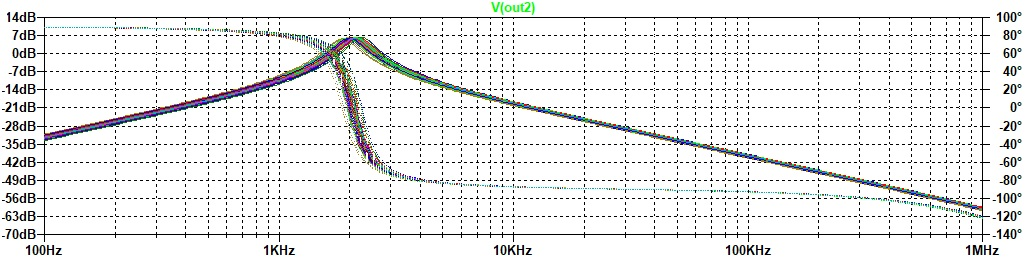
\includegraphics[scale = 0.7]{imagenes/ej1-montecarlo.jpg}
  \caption{An\'alsis de montecarlo (resistencias 5\%, capacitores 10\%)}
  \label{fig:1-montecarlo}
\end{figure*}

El valor elegido para $R$ fue $2.2k\Omega$. Los par\'ametros del circuito quedan determinados entonces de la siguiente manera:


\begin{table}[H]
	\centering

	\begin{tabular}{|c|c|c|c|}
		\hline
		           		& Valor ideal                              & Valor elegido                      	& Error ($\%$) 	\\ \hline \hline
		$R_1$      		& $2.2k\Omega$                        & $2.2k\Omega$                       	& 0            	\\ \hline
		$C_2$      		& $34.965nF$				& $34.878nF$               		& -0.25         	\\ \hline
		$R_3$      		& $2.2k\Omega$                        & $2.2k\Omega$                       & 0            	\\ \hline
		$R_4$      		& $2.2k\Omega$                        & $2.2k\Omega$                       & 0            	\\ \hline
		$R_8$      		& $2.2k\Omega$                        & $2.2k\Omega$                       & 0            	\\ \hline
		$C_6$      		& $34.965nF$ 				& $34.878nF$               		& -0.25         	\\ \hline
		$R_6$      		& $8.8k\Omega$                      	& $8.8k\Omega$       			& 0            	\\ \hline
		$\omega_0$ 	& $13,000\nicefrac{rad}{s}$	&  $13,032 \nicefrac{rad}{s}$ 	& 0.25         	\\ \hline
		$Q$        		& 4                                           & 4                              		& 0            	\\ \hline
	\end{tabular}
	\caption{Valores de los componentes, y $\omega_0$ y $Q$ resultantes}
\end{table}



De esta forma, todas las resistencias tienen su valor te\'orico exacto (dejando de lado la tolerancia del componente por el momento), y s\'olo se requiere hacer una combinaci\'on paralelo de $12k\Omega$ con $33k\Omega$ para obtener el valor de $R_6$. En cuanto a los capacitores, el valor de $34.878nF$ se obtiene al conectar en serie un capacitor de $39nF$ con uno de $330nF$. Tanto $C_2$ como $C_6$ afectan a $\omega_0$ con una sensibilidad de $-\nicefrac{1}{2}$, con lo cual sus efectos combinados s\'olo resultan en un $0.25\%$ de desviaci\'on respecto de $\omega_0$. En cuanto al valor de $Q$, al ser iguales ambos capacitores sus efectos se compensan, y s\'olo depende de $R_6$, con lo cual se obtiene de forma exacta.  \par

Con esta selecci\'on de componentes y operacional, se efectu\'o un an\'alisis de Montecarlo en \textit{LtSpice}. De acuerdo al mismo, la tolerancia de los componentes lleva a que el rango donde se encontrar\'a la frecuencia de corte es aproximadamente entre $1.85kHz$ y $2.3kHz$, lo cual implica un margen de error de $\pm 10\%$. \par

Por lo tanto, se procedi\'o a implementar este filtro en una PCB con los componentes indicados y el amplificador TL082. Se utilizaron resistencias de metal-film y capacitores film. A su vez, se incluyeron dos capacitores de $100nF$ multicapa de desacople: uno entre $V_{CC}^+$ y tierra y otro entre $V_{CC}^-$ y tierra. Estos capacitores tienen como funci\'on compensar peque\~nos cambios de tensi\'on en la alimentaci\'on del operacional, para que la misma sea m\'as estable.


\section{An\'alisis de resultados}

\subsection{Respuesta en frecuencia}

\begin{figure*}[h!]
	\centering
  	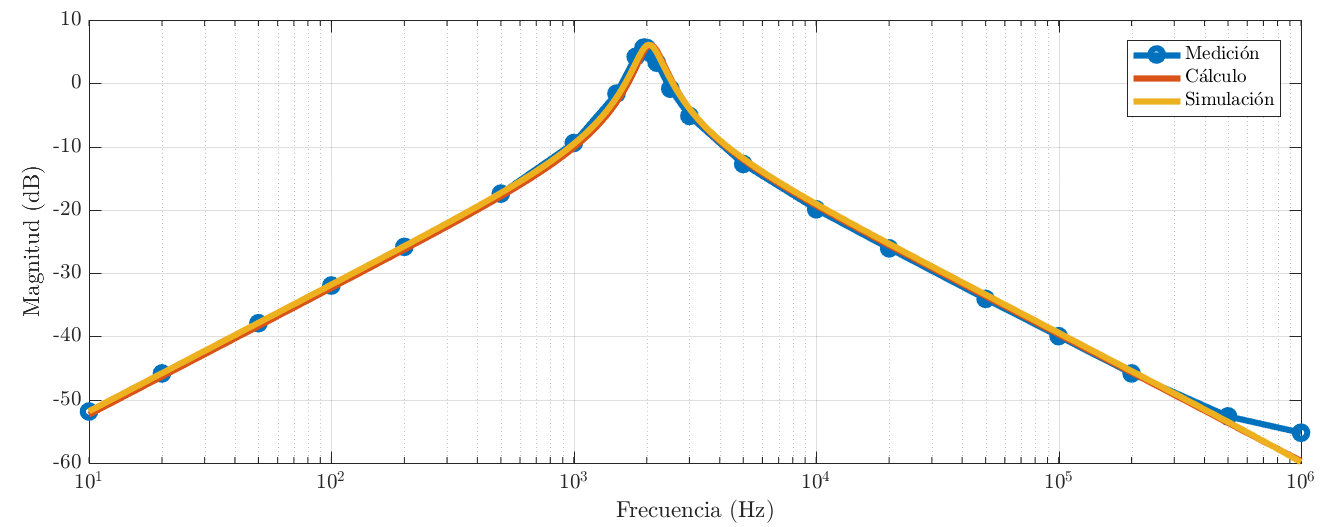
\includegraphics[scale = 0.5]{imagenes/tc_tp3_ej1_hf_mag.png}
  	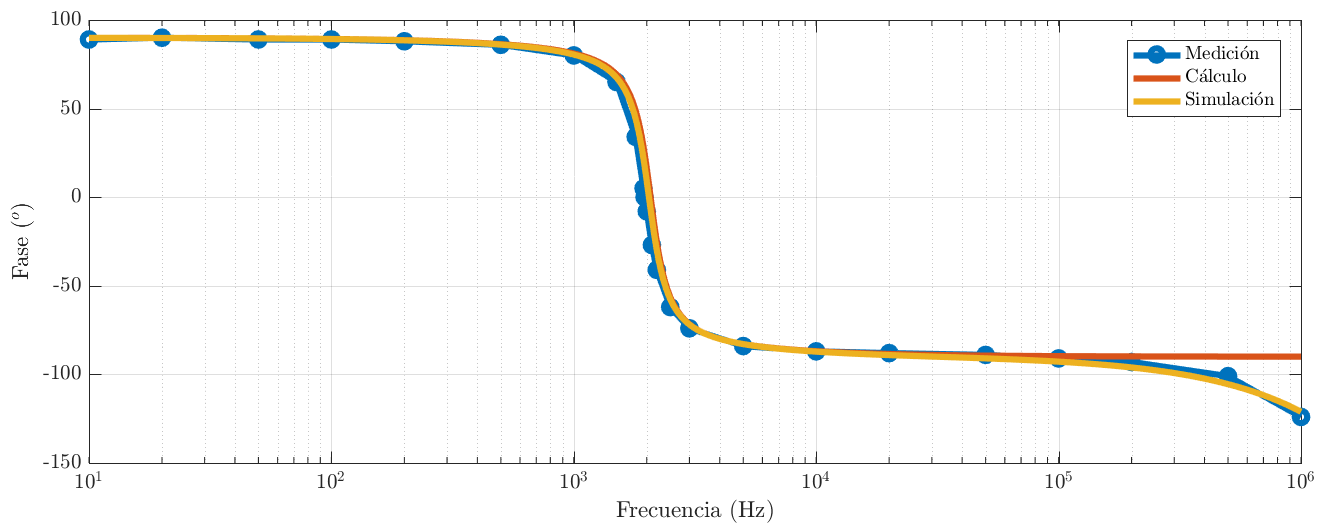
\includegraphics[scale = 0.5]{imagenes/tc_tp3_ej1_hf_fase.png}
  	\caption{Diagrama de bode de la respuesta en frecuencia}
  	\label{fig:1-rtafrec}
\end{figure*}

Como se observa en los gr\'aficos de la figura (\ref{fig:1-rtafrec}), la respuesta en frecuencia del circuito coincide con la que se obtiene en la simulaci\'on. Para frecuencias altas, a partir de $100kHz$, comienzan a observarse en la fase los efectos del polo del operacional, que no se tuvieron en cuenta a la hora de calcular la funci\'on transferencia. Por otro lado, la medici\'on de magnitud a $1MHz$ discrepa de tanto la simulaci\'on como el c\'alculo. Esto puede deberse a que debido a la gran atenuaci\'on, la se\~nal de salida era tan peque\~na que resulta comparable con el ruido del osciloscopio, eliminando su validez. Tambi\'en es posible que a estas frecuencias, el comportamiento de los componentes se vea afectado por sus partes inductivas, lo cual no est\'a contemplado en el modelo te\'orico ni en \textit{Spice}. \par

Se observa una pendiente de +20dB por d\'ecada hasta la frecuencia de corte, alrededor de los $2k\Omega$, y -20dB por d\'ecada a partir de la misma, con un salto de $-180^\circ$ en la fase: de $90^\circ$ a $-90^\circ$. Siendo que el factor de calidad calculado es $Q=4$, y se observa en la medici\'on el mismo comportamiento que en la simulaci\'on y el c\'alculo, se puede concluir que el filtro cumple con las prestaciones requeridas. 

\subsection{Respuesta al escal\'on}

\todo[inline]{calcular y simular rta esc}

De lo desarrollado en la secci\'on anterior, podr\'iamos preguntarnos si el circuito exhibir\'a el comportamiento de derivador para frecuencias mucho menores que la de resonancia, y de integrador para frecuencias mucho mayores. En esos rangos, el filtro tiene la pendiente y la fase adecuada para que esto suceda. Se realizaron pues mediciones de respuesta al escal\'on. Para la derivada, deber\'iamos observar s\'olo el transitorio cuando la entrada tiene un salto, donde la derivada es el impulso $\delta(t)$, y en el integrador deber\'iamos observar una se\~nal triangular.

Calcularemos primero anal\'iticamente qu\'e deber\'ia observarse a la salida. Siendo que ya contamos con la funci\'on transferencia del sistema (\ref{eq:voutvin}) y que el mismo es BIBO-estable (pues la parte real de sus ceros es negativa, como se observa en el diagrama de polos (\ref{fig:1-polos})), para obtener la respuesta al escal\'on basta antitransformar la expresi\'on:

\[	Y(s) = H(s) \cdot \mathcal{L}\{u(t)\{(s) = \frac{H(s)}{s} \Leftrightarrow\]\\
\[	Y(s) =  \frac{\left( 1+\frac{R_4}{R_8} \right) \cdot \frac{L_{GIC}}{R_6}}{ LC_6 \cdot s^2  + \frac{L_{GIC}}{R_6} \cdot s + 1} \]

Si reemplazamos por los par\'ametros de este circuito $\alpha = \frac{1}{2R_6 C_6}$ (coeficiente de amortiguamiento) y $\omega_d = \sqrt{\omega_0^2 - \alpha^2}$ (pseudofrecuencia, que es real porque los polos del sistema son complejos conjugados), entonces podemos reescribir la salida del sistema completando cuadrados y asociando como:\par

\[
	\begin{aligned} 
	Y(s) &= \frac{ \left( 1+\frac{R_4}{R_8} \right) \cdot \frac{L_{GIC}}{R_6} \cdot \frac{1}{L_{GIC}C_6} }{s^2  + \frac{1}{2R_6 C_6} \cdot s + \frac{1}{L_{GIC}C_6}} \\
	 &= \left( 1+\frac{R_4}{R_8} \right) \cdot \frac{2\alpha}{\omega_d} \cdot \left( \frac{\omega_d}{(s+\alpha)^2 + \omega_d^2} \right)
	 \end{aligned}
\]

Recordando que $\mathcal{L}\{ \frac{b}{(s+a)^2+b^2} \}(s) = e^{-at}\cdot \cos{bt}$, entonces por linealidad la respuesta al escal\'on de este circuito es:

\begin{equation}
	y(t) = \left(1+\frac{R_4}{R_8} \right) \cdot \frac{2\alpha}{\omega_d} \cdot e^{-\alpha t}\cdot \cos{\omega_d t}
\end{equation} 

Por lo tanto, el transitorio que esperar\'iamos observar es una oscilaci\'on modulada por una exponencial decreciente, con pseudofrecuenica $\omega_d \sim 11,286 \nicefrac{rad}{s} \sim 1,800Hz$ y tiempo caracter\'istico $\tau = \frac{1}{\alpha} \sim 153\mu s$. Por lo tanto, el tiempo de establecimiento de la se\~nal deber\'ia ser de aproximadamente $6\tau \sim 0.92ms$, o el equivalente a 1.65 pseudoper\'iodos.

\begin{figure}[H]
	\centering
  	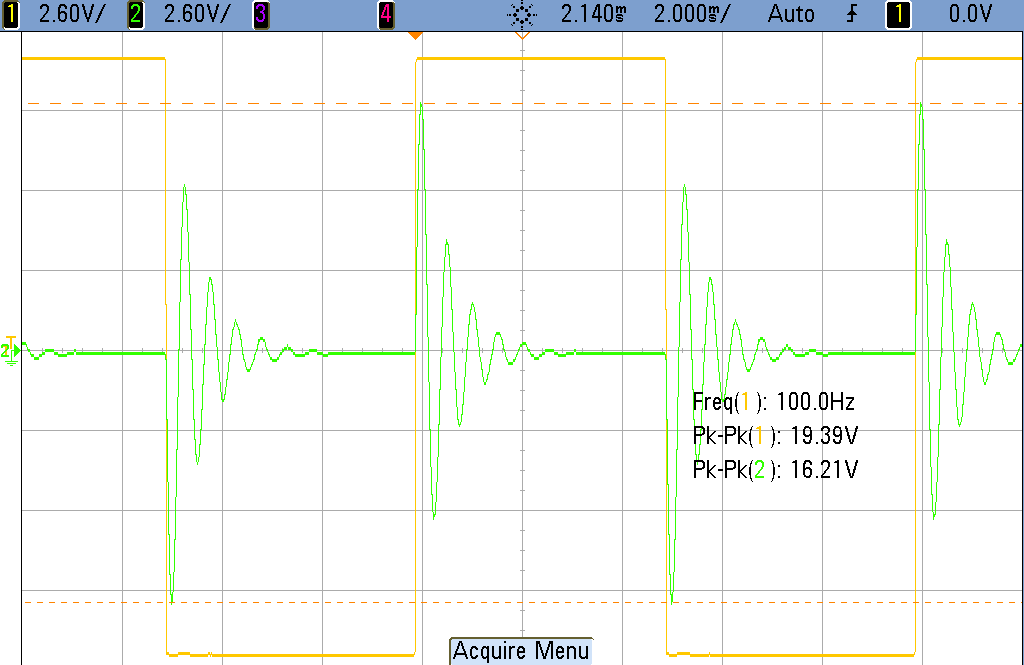
\includegraphics[scale = 0.3]{imagenes/tc_tp3_ej1_100Hz.png}
  	\caption{Respuesta a escal\'on de 100Hz}
  	\label{fig:1-rtaesc-100Hz}
\end{figure}

Se observa aqu\'i que si bien la forma del transitorio es la que se esperaba obtener, su tiempo de establecimiento es pr\'acticamente el doble que el calculado. Esto puede deberse a
\todo[inline]{terminar esto, simular}


En esta frecuencia, observamos que una vez superado el r\'egimen permanente, la se\~nal se establece en $0V$, lo cual coincide con el comportamiento esperado. Sin embargo, la duraci\'on del transitorio es del orden de la frecuencia. Para que este tiempo sea menos significante, deber\'iamos trabajar en frecuencias menores, pero esto a su vez conllevar\'ia una atenuaci\'on cada vez mayor. Por lo tanto, no ser\'ia prudente usar este circuito como derivador.

\begin{figure}[H]
	\centering
  	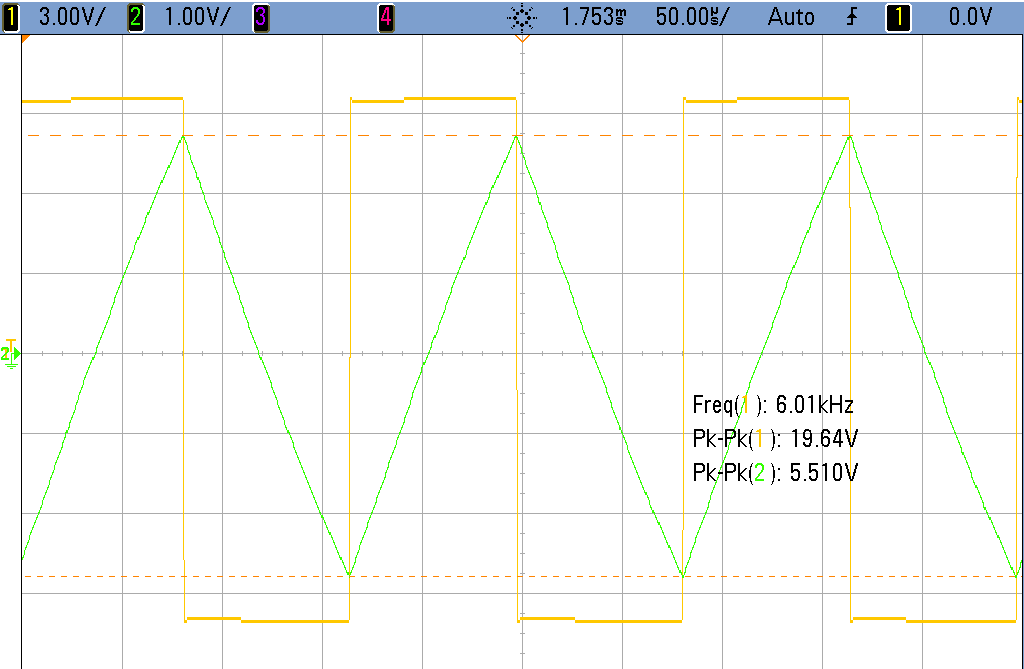
\includegraphics[scale = 0.3]{imagenes/tc_tp3_ej1_6kHz.png}
  	\caption{Respuesta a escal\'on de 6kHz}
  	\label{fig:1-rtaesc-6kHz}
\end{figure}

Con una frecuencia de $6kHz \sim 3\cdot f_0$, en la salida ya se observa la integral de la entrada, que es lo que esper\'abamos observar. Recordando que la fase comienza a  verse afectada por los polos del operacional a partir de los $100kHz$ aproximadamente, este circuito podr\'ia usarse como integrador para se\~nales de frecuencias entre los $6kHz$ y los $100kHz$.

\begin{figure*}[h!]
	\centering
  	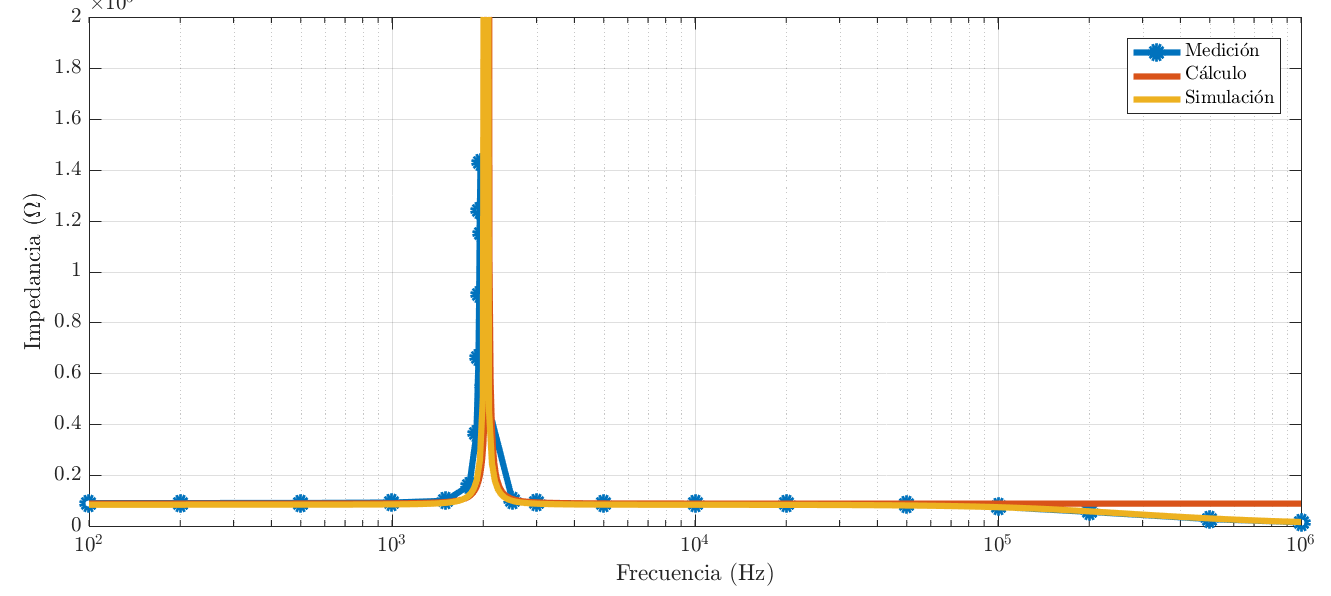
\includegraphics[scale = 0.5]{imagenes/tc_tp3_ej1_zin_x1_mag.png}
  	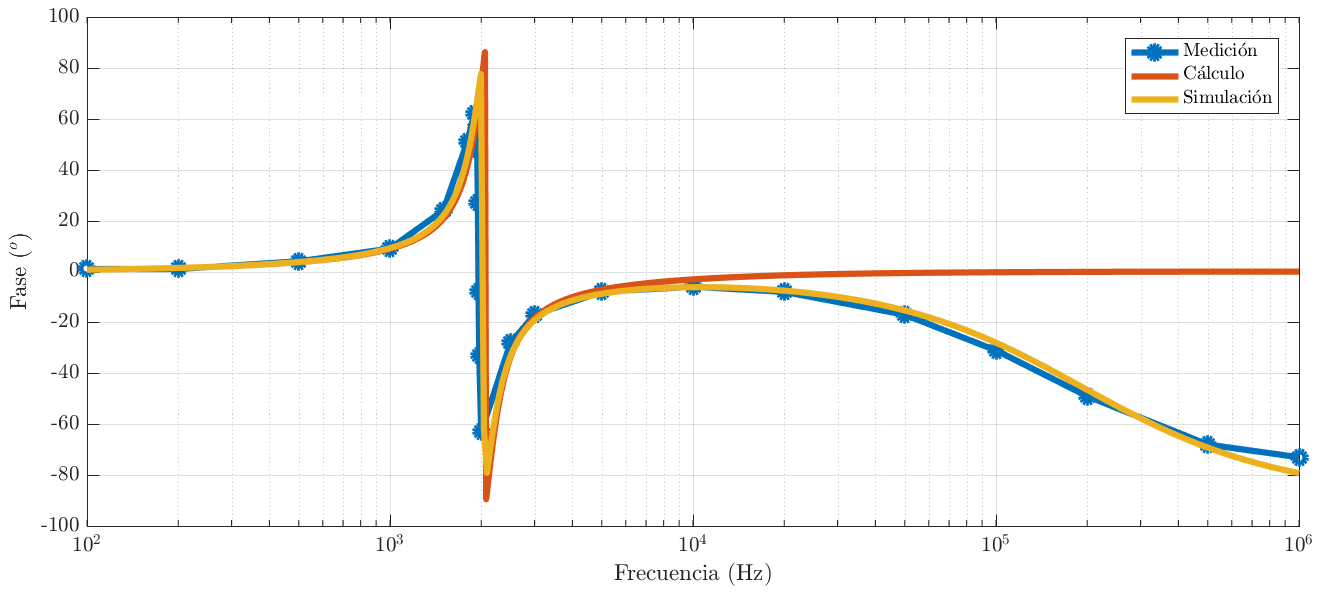
\includegraphics[scale = 0.5]{imagenes/tc_tp3_ej1_zin_x1_fase.png}
  	\caption{Diagrama de bode de la impedancia de entrada}
  	\label{fig:1-zin}
\end{figure*}


\subsection{Impedancia de entrada}


Si consideramos la simplificaci\'on del GIC a una bobina de la figura (\ref{fig:ej1-rlc}), la impedancia de entrada del circuito no es m\'as que una resistencia en serie con una bobina y un capacitor en paralelo. Operando algebr\'aicamente la expresi\'on de la impedancia de entrada que se obtiene es:

\begin{equation}
	Z_{in}(s) = R_6 \cdot \left( \frac{L_{GIC}C_6 \cdot s^2 + \frac{L_{GIC}}{R_6} \cdot s + 1}{L_{GIC}C_6 \cdot s^2 +1} \right) 
\end{equation}

Por lo tanto, esperar\'iamos que la impedancia de entrada presente un pico en la frecuencia de resonancia, donde idealmente deber\'ia tenerse impedancia infinita, y que para frecuencias mucho mayores o mucho menores se observe $Z_{in}(f) \sim R_6 = 8.8k\Omega$.\par

Sin embargo, como se observa en el diagrama de bode de la figura (\ref{fig:1-zin}), esta expresi\'on no es suficiente para explicar el comportamiento del circuito. Si bien mediciones y c\'alculo coinciden hasta los $10kHz$ la fase y $100kHz$ en la magnitud, es necesario tener en cuenta la presencia de las puntas del osciloscopio para poder tener un modelo representativo de lo que est\'a sucediendo, como se observa en la simulaci\'on. En esta \'ultima est\'an incluidos los efectos de las dos puntas conectadas para medir la impedancia de entrada: una antes de una resistencia de $8.9k\Omega$ (medida con mult\'imetro), y otra entre esta resistencia y el circuito, considerando a la impedancia de entrada como el cociente de la tensi\'on de entrada al circuito y la corriente por esta resistencia.


\subsection{Impedancia de salida}

\begin{figure*}[h!]
	\centering
  	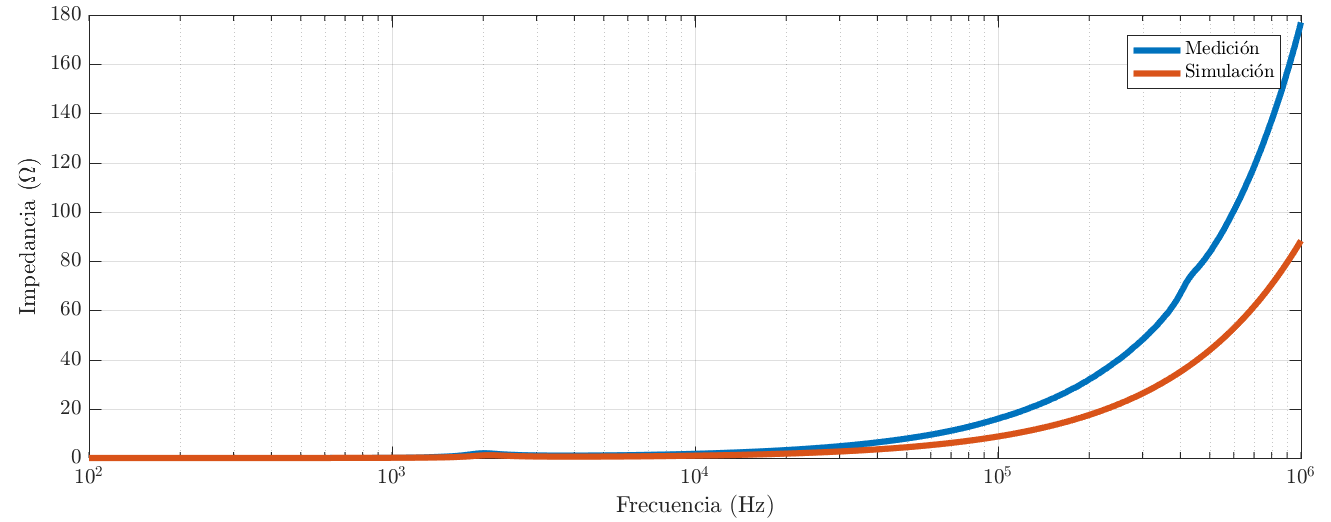
\includegraphics[scale = 0.5]{imagenes/tc_tp3_ej1_zout_mag.png}
  	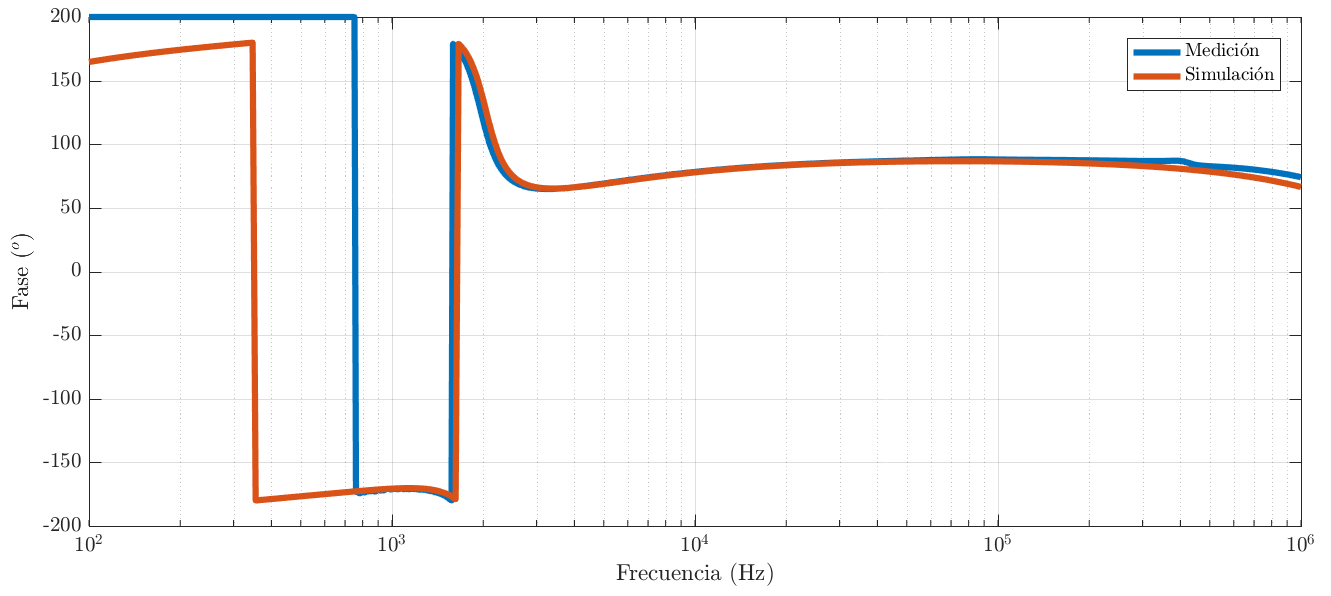
\includegraphics[scale = 0.5]{imagenes/tc_tp3_ej1_zout_fase.png}
  	\caption{Diagrama de bode de la impedancia de salida}
  	\label{fig:1-zout}
\end{figure*}

La impedancia de salida de este circuito es la salida del uno de los \textit{op amps} del TL082, y como tal idealmente es nula. Sin embargo, simulando en \textit{LtSpice} se puede observar que si bien la misma es de unos pocos miliohms para frecuencias bajas, a partir de los $10kHz$ comienza a crecer, llegando a aproximadamente $90\Omega$ en $1MHz$. En este caso las mediciones se realizaron con un analizador de impedancias para no tener problemas con las puntas del osciloscopio. \par

Incluso utilizando el analizador de impedancias, la magnitud de la impedancia de salida era tan peque\~na que el instrumento no lograba medir su fase. S\'olo a partir de aproximadamente $750Hz$, cuando se super\'o el medio ohm, se comenzaron a obtener datos sobre la misma. \par

Como se puede observar en la figura (\ref{fig:1-zout}), en el rango de valores donde la fase pudo medirse, la misma coincide con la de la simulaci\'on, y muestra un salto de aproximadamente $120^\circ$ alrededor de la frecuencia de resonancia. Por otro lado, la magnitud coincide en forma, mas no as\'i en valor: se midi\'o consistentemente casi el doble de lo que predice la simulaci\'on. Esto puede deberse a discrepancias entre el modelo utilizado por \textit{Spice}, y el operacional concreto utilizado. Si bien cada modelo tiene caracter\'isticas gen\'ericas similares, algunos par\'ametros pueden poseer una gran dispersi\'on, como es por ejemplo el caso de $A_0$. \par 

Siendo que observamos un salto en la fase alrededor de la frecuencia de corte, ser\'ia razonable que esto se vea reflejado en la magnitud de la impedancia. Si bien no es apreciable en la escala de la figura (\ref{fig:1-zout}), al hacer \textit{zoom} alrededor de $f_0$ efectivamente se aprecia un pico en la impedancia, similar al que se ve\'ia a la entrada. Esto pone de manifiesto el comportamiento no ideal del operacional, puesto que al no ser su impedancia de salida verdaderamente 0, la del circuito ya no es s\'olo la del operacional sino \'esta en paralelo con la salida del resto del circuito. 

\begin{figure}[H]
	\centering
  	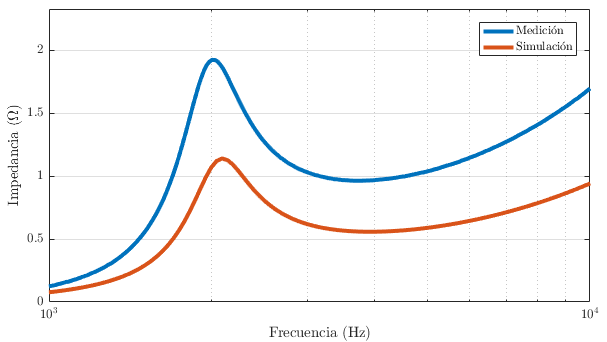
\includegraphics[scale = 0.6]{imagenes/tc_tp3_ej1_zout_zoom.png}
  	\caption{Detalle de la impedancia de salida alrededor de $f_0$}
  	\label{fig:1-zout-zoom1}
\end{figure}


\subsection{Limitaciones}

\subsubsection{Limitaciones por tensi\'on}

Como ya se ha discutido, si bien este circuito puede modelarse como un RLC, no se utiliza una bobina sino una combinaci\'on de resistencias, capacitores y operacionales. Por lo tanto, su comportamiento ser\'a el deseado siempre y cuando estos \'ultimos est\'en trabajando en su zona lineal, para lo cual es fundamental evitar que lleguen a saturaci\'on. \par

Debido a que los operacionales se alimentaron con $V_{cc}^\pm = \pm 15V$, ser\'ia prudente dejar al menos $3V$ de margen, es decir no permitir que la salida deba superar los $24V_{pp}$. 

\begin{figure}[H]
	\centering
  	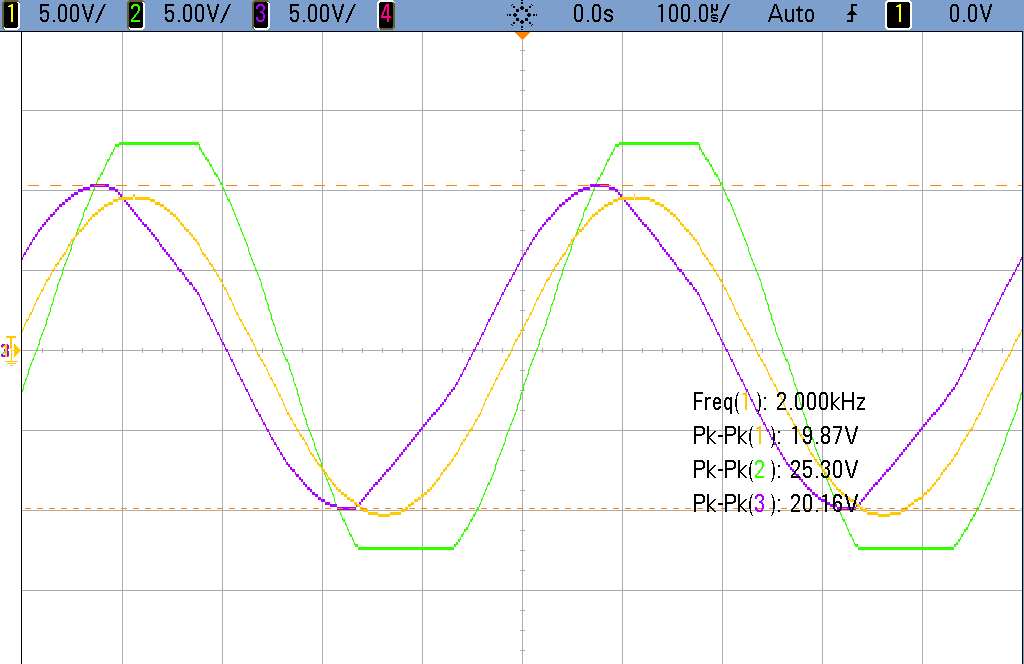
\includegraphics[scale = 0.3]{imagenes/tc_tp3_ej1_saturacion.png}
  	\caption{Salida del circuito con el \textit{op amp} saturado}
  	\label{fig:1-saturacion}
\end{figure}

Se observa aqu\'i que la m\'axima tensi\'on pico a pico que puede haber a la salida es $25.3V_{pp}$, por lo cual mantenerlo en $24V_{pp}$ ser\'ia recomendable.\par

Debe tenerse en cuenta, adem\'as, que la salida de los dos operacionales describen dos comportamientos distintos, por lo cual que uno no sature no implica que el otro no lo haga. En la figura (\ref{fig:1-saturacion}) se aprecia que con que uno s\'olo de los operacionales sature (en $V_{out}$, la se\~nal verde) lleva a que el otro ($V_1$, se\~nal violeta) tampoco exhiba el comportamiento deseado. Recordando los resultados obtenidos en (\ref{eq:v1v2vgic}) y (\ref{eq:1-vgicvin}), as\'i como la expresi\'on de $L_{GIC} $ en funci\'on de los componentes en (\ref{eq:1-LGIC}) podemos obtener la transferencia al otro operacional como:

\begin{equation}
	\frac{V_1}{V_{in}} (s)=  - \frac{\nicefrac{R_1}{R_6}}{ L_{GIC}C_6 \cdot s^2  + \frac{L_{GIC}}{R_6} \cdot s + 1}
\end{equation}

Esto corresponde a un filtro pasabajos de segundo orden, cuya frecuencia de corte es la misma que la de resonancia del circuito. Por lo tanto, para frecuencias bajas se deber\'a tener en cuenta la saturaci\'on de este \textit{op amp} en lugar de la salida del circuito, puesto que la ganancia se estabilizar\'a en $\nicefrac{R_1}{R_6} = \nicefrac{1}{4}\sim -12dB$ en lugar de decrecer 20dB por d\'ecada. Sin embargo, esto no pudo observarse con los $20V{pp}$ m\'aximos que entregan los generadores del laboratorio de la Universidad.

\section{Conclusiones}

\end{document}
